\section{酸的通性 pH值}\label{sec:5-4}

就人类认识事物的过程来说,总是由认识个别的和特殊的事物,逐步地扩大到认识一般的事物。
我们在学习了几种个别的酸的性质以后,就要逐步地扩大到认识酸的一般性质。

\subsection{酸的分类和命名}

根据酸的分子里是不是含有氧原子,可以把酸分成含氧酸和无氧酸两类。
硫酸、硝酸、磷酸、碳酸等是含氧酸,盐酸、氢硫酸(\ce{H2S})等是无氧酸。

根据酸分子电离时所能生成的氢离子的个数,可以把酸分成一元酸、二元酸、三元酸等。
例如,盐酸是一元酸,硫酸是二元酸,磷酸是三元酸。

含氧酸一般是根据它的分子里氢氧两元素以外的另一种元素的名称而命名为 “某酸”。
例如,\ce{H2SO4} 叫硫酸, \ce{HClO3} 叫氯酸, \ce{H3PO4} 叫磷酸等等。
无氧酸的命名,是在氢字的后面加上另一元素的名称,叫做 “氢某酸” 。
例如,\ce{HCl} 叫做氢氯酸(俗名盐酸), \ce{H2S} 叫做氢硫酸,等等。


\subsection{酸的通性}

由于酸在水溶液里都能电离,生成氢离子,所以,它们有一些相似的化学性质。

1. 酸溶液能跟酸碱指示剂起反应。例如,紫色的石蕊试液遇酸变红色,无色的酚酞试液遇酸不变色。

2. 酸能跟多种活泼金属起反应,通常生盐和氢气。

我们已经知道,锌和铁能分别跟盐酸起置换反应,生成氢气和相应的盐。
\begin{fangchengshi}
    \ce{ Zn + 2HCl = ZnCl2 + H2 ^ } \\[-0.5em]
    \ce{ Fe + 2Hcl = FeCl2 + H2 ^ }
\end{fangchengshi}

在这两个反应里,每个锌和铁的原子失去两个电子,它们的化合价都由 $0$ 价上升为 $+2$ 价,
每个氢原子接受一个电子,化合价由 $+1$ 价下降为 $0$ 价。这两个反应都属于氧化-还原反应。

是不是各种金属都能跟酸起置换反应呢?

\begin{shiyan}
    把铜和银各一小片分别放入盛有稀盐酸的两个试管里,观察有没有反应发生。
\end{shiyan}

由实验看出,铜和银跟稀盐酸不起反应,可见,金属跟酸反应与金属的性质有关。
经过长期的实践,人们总结出常见金属的化学活动性顺序如下:
\begin{center}
    \begin{tblr}{columns={c}}
        \ce{K} & \ce{Ca} & \ce{Na} & \ce{Mg} & \ce{Al} & \ce{Zn} & \ce{Fe}  & \ce{Sn} & \ce{Pb} & \ce{(H)} & \ce{Cu} &  \ce{Hg} & \ce{Ag} & \ce{Pt} & \ce{Au} \\
       \SetCell[c=15]{c} \tikz[overlay, >=Stealth] \draw [->] (-4, 0.5) -- (8.5, 0.5); 金属活动性由强逐渐减弱
    \end{tblr}
\end{center}
% \begin{center}
%     \begin{tblr}{columns={c}}
%         \ce{K}  \ce{Ca} \ce{Na} \ce{Mg} \ce{Al} \ce{Zn} \ce{Fe} \ce{Sn} \ce{Pb} \ce{(H)} \ce{Cu} \ce{Hg} \ce{Ag} \ce{Pt} \ce{Au} \\
%         \tikz[overlay, >=Stealth] \draw [->] (-2, 0.5) -- (6.5, 0.5); 金属活动性由强逐渐减弱
%     \end{tblr}
% \end{center}
% K Ca Na Mg Al Zn Fe Sn Pb (H) Cu Hg Ag Pt Au


\begin{wrapfigure}[23]{r}{4cm}
    \centering
    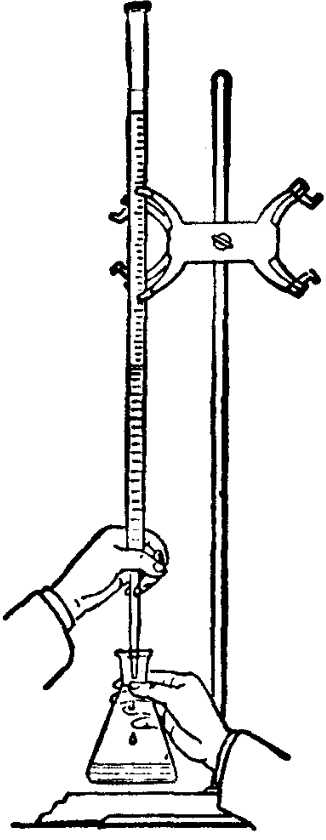
\includegraphics[width=3cm]{../pic/czhx1-ch5-3}
    \caption{\begin{minipage}[t]{2.5cm}
        用滴定管做\\
        中和反应实验
    \end{minipage}}\label{fig:5-3}
\end{wrapfigure}

在金属活动性顺序中,金属的位置越靠前,金属在水溶液中就越容易失去电子变成离子,它的活动性就越强。
在上列金属中,钾的活动性最强,钙次之,金的活动性最弱。排在氢前面的金属能置换出酸里的氢,
排在氢后面的金属不能置换出酸里的氢。

3. 酸能跟某些金属氧化物起反应,生成盐和水。例如:
\begin{fangchengshi}
    \ce{ CuO + H2SO4 = CuSO4 + H2O }
\end{fangchengshi}

4. 酸能跟某些盐起反应,生成另一种酸和另一种盐。例如:
\begin{fangchengshi}
    \ce{ AgNO3 + HCl = AgCl v + HNO3 }
\end{fangchengshi}


5. 酸跟碱起中和反应,生成盐和水。

\begin{shiyan}
    在盛有氢氧化钠溶液的锥形瓶里,滴入几滴酚酞试液,溶液变成红色。
    再用滴定管慢慢滴入稀盐酸,同时不断振荡溶液,一直到溶液刚刚变成无色为止(图 \ref{fig:5-3}) 。
\end{shiyan}

酚酞试液遇碱溶液变成红色,当滴入盐酸到酚酞试液刚刚变成无色时,溶液既不显酸性,也不显碱性。反应可用下式表示:
\begin{fangchengshi}
    \ce{ NaOH + HCl = NaCl + H2O }
\end{fangchengshi}

\zhongdian{酸跟碱作用而生成盐和水的反应,叫做中和反应。}

中和反应在工农业生产和科学实验中应用很广。例如,
在化工生产和科学实验里,当溶液里有过量酸或碱时,常用适量的碱或酸来中和;
在农业生产上,强酸性的土壤不适宜植物的生长,可以施入适量的熟石灰〔\ce{Ca(OH)2}〕来中和土壤里的酸,
就可以改良土壤,改善作物的生长条件。


\subsection{pH 值 —— 酸碱度的表示法}

在前边做过的实验里,我们曾用酸碱指示剂来试验溶液里是否含有酸或碱,也就是说,试验溶液是酸性还是碱性。
但是,在工农业生产和科学实验中,仅知道溶液是酸性还是碱性是不够的。还必须测定和控制溶液的酸碱性强弱程度,即溶液的酸碱度。

溶液的酸碱度常用 pH 值来表示,pH 值的范围通常在 0—14 之间(图 \ref{fig:5-4})。

\begin{figure}[htbp]
    \centering
    \begin{tikzpicture}[scale=0.8, >=Stealth,
    every node/.style={fill=white, inner sep=1pt},
]
    \draw (-0.5, 0) -- (14.5, 0);
    \foreach \x in {0, 1, ..., 14} {
        \ifnum \x = 7
            \draw (\x, -0.5) -- (\x, 0.4) node [above=0.1em] {$\x$};
        \else
            \draw (\x, 0) -- (\x, 0.2) node [above=0.2em] {$\x$};
        \fi
    }

    \draw [<->, very thick] (0.5, -1) -- (13.5, -1)
        node [midway] {中性}
        node [pos=0.2, below=0.5em] {酸性增强}
        node [pos=0.8, below=0.5em] {碱性增强};
\end{tikzpicture}


    \caption{pH 值和酸碱性}\label{fig:5-4}
\end{figure}

$\text{pH 值} = 7$ 时,溶液呈中性,\ce{H+} 离子和 \ce{OH-} 离子浓度相等。

$\text{pH 值} < 7$ 时,溶液呈酸性, pH 值越小,\ce{H+} 离子浓度越大,酸性越强。

$\text{pH 值} > 7$ 时,溶液呈碱性, pH 值越大,\ce{OH-} 离子浓度越大,碱性越强。

测定 pH 值的最简便的方法是使用 pH 试纸,这种试纸在不同酸碱度的溶液里,显示不同的颜色。
测定时,把待试溶液滴在 pH 试纸上,然后把试纸显示的颜色跟标准比色卡对照,便可知道溶液的 pH 值。
如果要精确地测定溶液的 pH 值,可以采用一种叫 pH 计的仪器。

\begin{shiyan}
    配制几种不同浓度的酸和碱的稀溶液,用 pH 试纸测定它们的 pH 值。
\end{shiyan}

\begin{shiyan}
    取 2 克土壤样品放在表面皿上,加蒸馏水 3 毫升,搅拌一分钟,静置澄清。用 pH 试纸测溶液的 pH 值。
\end{shiyan}

了解溶液的酸碱度,对工农业生产有重要的意义。例如,
在化工生产中,许多反应必须在一定酸碱度的溶液里才能进行。
在农业方面,土壤酸碱度的大小,对作物的生长也有很大的影响。
一般说来,大多数的作物适宜在中性或接近中性的土壤中生长。
当土壤的 pH 值小于 4 或大于 $8.5$ 时,一般作物难于生长。



\begin{xiti}

\xiaoti{把足量的稀硫酸加入盛有少量氧化铜和铜的混和物的试管里,加热后过滤,在滤纸上剩下什么物质?在滤液里有什么物质?}

\xiaoti{有两瓶溶液,一瓶溶液的 pH 值是 $4.5$, 另一瓶溶液的 pH 值是 $9.5$。在这两瓶溶液里,各滴入几滴酚酞试液,有什么现象发生?
    如果要使前一种溶液的 pH 值升高,后一种溶液的 pH 值降低,可以采取什么措施?
}

\xiaoti{某工厂化验室用 $15\%$ 的氢氧化钠溶液,洗涤一定量石油产品中的残余硫酸,共消耗这种溶液 40 克,
    洗涤后溶液呈中性,问在这一定量的石油产品里含硫酸多少克?
}

\xiaoti{把锌和铜的混和物 50 克和足量稀硫酸起反应,可制得氢气 $1.1$ 克,求这混和物里含锌和铜各多少克?}


\xiaoti{在家里用石灰水(碱性)、食醋(酸性)来试验一些植物色素,如红紫色的花瓣、果皮等,
    看它们的颜色发生什么变化。(如果用花瓣、果皮的汁液或酒精浸出液来试验,效果可以更好些。)
}

\end{xiti}

